\documentclass[hyperref={breaklinks,colorlinks,
   urlcolor=blue,citecolor=blue,linkcolor=red}]{beamer}
   \setbeamercolor{section in head/foot}{bg=black}
   

\definecolor{GUblue}{RGB}{0, 0, 140} %b204,b153
\definecolor{mayablue}{rgb}{0.45, 0.76, 0.98}
\definecolor{lightcornflowerblue}{rgb}{0.6, 0.81, 0.93}
\usecolortheme[named=GUblue]{structure}


\mode<presentation>
{
  \usetheme{Ilmenau} %Madrid, AnnArbor, Goettingen, Warsaw,CambridgeUS
  %\usecolortheme{seahorse} %whale, beaver,rose,crane, wolverine
  \usefonttheme{serif}
  
} 


\setbeamertemplate{frametitle continuation}{}

\newcommand{\backupbegin}{
   \newcounter{finalframe}
   \setcounter{finalframe}{\value{framenumber}}
}
\newcommand{\backupend}{
   \setcounter{framenumber}{\value{finalframe}}
}

\usepackage[round]{natbib}
\usepackage{amsmath}
\usepackage{graphicx}
\usepackage{verbatim}
\usepackage[english]{babel}
\usepackage[absolute,overlay]{textpos}
\usepackage{caption}
\captionsetup{font=scriptsize}
\usepackage{amssymb}
\usepackage{tcolorbox}
\usepackage{tipa}
\usepackage{booktabs}
\usepackage{siunitx}
\usepackage{adjustbox}
\usepackage{setspace}
\usepackage{lipsum}
\usepackage{physics}
\usepackage{qrcode}
\renewcommand{\vec}[1]{\boldsymbol{#1}}
\newcommand{\Hmns}{\tiny\textrm{H}}
\usepackage{media9}
\usepackage{aasmacros}
\usepackage{multimedia}
\usepackage{sidecap}
\usepackage{tikz}
\usetikzlibrary{arrows,positioning}

\setbeamertemplate{caption}[numbered]{\centering\raggedright}


\newcommand\FourQuad[4]{%
    \begin{minipage}[b][.35\textheight][t]{.47\textwidth}#1\end{minipage}\hfill%
    \begin{minipage}[b][.35\textheight][t]{.47\textwidth}#2\end{minipage}\\[0.5em]
    \begin{minipage}[b][.35\textheight][t]{.47\textwidth}#3\end{minipage}\hfill
    \begin{minipage}[b][.35\textheight][t]{.47\textwidth}#4\end{minipage}%
}


\usepackage{xspace}
\newcommand{\bilby}{{\sc Bilby}\xspace}
\newcommand{\PyCBC}{{\sc PyCBC}\xspace}
\newcommand{\IPython}{{\sc IPython}\xspace}
\newcommand{\Python}{{\sc Python}\xspace}
\newcommand{\Numpy}{{\sc NumPy}\xspace}
\newcommand{\astropy}{{\sc Astropy}\xspace}
\newcommand{\gwpy}{{\sc GWpy}\xspace}
\newcommand{\lal}{{\sc LALSimulation}\xspace}



\usepackage{etoolbox}

\makeatletter

% Patch case where name and year are separated by aysep
\patchcmd{\NAT@citex}
  {\@citea\NAT@hyper@{%
     \NAT@nmfmt{\NAT@nm}%
     \hyper@natlinkbreak{\NAT@aysep\NAT@spacechar}{\@citeb\@extra@b@citeb}%
     \NAT@date}}
  {\@citea\NAT@nmfmt{\NAT@nm}%
   \NAT@aysep\NAT@spacechar\NAT@hyper@{\NAT@date}}{}{}

% Patch case where name and year are separated by opening bracket
\patchcmd{\NAT@citex}
  {\@citea\NAT@hyper@{%
     \NAT@nmfmt{\NAT@nm}%
     \hyper@natlinkbreak{\NAT@spacechar\NAT@@open\if*#1*\else#1\NAT@spacechar\fi}%
       {\@citeb\@extra@b@citeb}%
     \NAT@date}}
  {\@citea\NAT@nmfmt{\NAT@nm}%
   \NAT@spacechar\NAT@@open\if*#1*\else#1\NAT@spacechar\fi\NAT@hyper@{\NAT@date}}
  {}{}

\makeatother

\defbeamertemplate*{footline}{myminiframes theme}
  {%
    \begin{beamercolorbox}[colsep=1.5pt]{upper separation line foot}
    \end{beamercolorbox}
    \begin{beamercolorbox}[ht=2.5ex,dp=1.125ex,%
      leftskip=.3cm,rightskip=.3cm plus1fil]{author in head/foot}%
      \leavevmode{\usebeamerfont{author in head/foot}\insertshortauthor}%
      \hfill%
      {\usebeamerfont{institute in head/foot}\usebeamercolor[fg]{institute in head/foot}\insertshortinstitute}%
    \end{beamercolorbox}%
    \begin{beamercolorbox}[ht=2.5ex,dp=1.125ex,%
      leftskip=.3cm,rightskip=.3cm plus1fil]{title in head/foot}%
      {\usebeamerfont{title in head/foot}\insertshorttitle\hfill \insertframenumber/\inserttotalframenumber}%<-here
    \end{beamercolorbox}%
    \begin{beamercolorbox}[colsep=1.5pt]{lower separation line foot}
    \end{beamercolorbox}
  }
\makeatother

\addtobeamertemplate{headline}{\hypersetup{linkcolor=.}}{}
\addtobeamertemplate{footline}{\hypersetup{linkcolor=.}}{}

\title[Hierarchical Geography]
{Hierarchical Geography with \Python}
\subtitle{A Very Brief Introduction}
\author[Gerald Leung]{Gerald Leung\inst{1}} %\\ Supervisor: Ik Siong Heng\inst{1}}
\institute[PHS Geospatial]{\inst{1}Public Health Scotland}%{\inst{1}School of Physics and Astronomy,\\ University of Glasgow}
\date[\today]{\today}
%\logo{\includegraphics[width=2.2cm]{emblem.jpg}}
%\titlegraphic{\includegraphics[scale=0.055]{emblem.jpg}}


%\logo{\includegraphics[scale=0.8]{SchPhyAst_colour.png}}

\begin{document}


\begin{frame}
\titlepage
%\vspace{-2cm}
%\begin{center}
%\includegraphics[width=0.40\textwidth]{SchPhyAst_colour.png}\includegraphics[width=0.30\textwidth]{cu_logo_4c_centre-eps-converted-to.pdf}
%\end{center}
\end{frame}




\section{Introduction}

\begin{frame}{Background}
\begin{itemize}
\item{We use GP boundaries as an example}
\begin{itemize}
\item{areas covered are defined with different geographies}
\item{e.g. postcode districts and sectors}
\item{ultimately we are only interested in the overall boundary of a GP}
\end{itemize}
\item{How do we merge geographies at different levels?}
$\Longrightarrow \textrm{\texttt{GeoPandas} in \Python}$
\end{itemize}
\end{frame}

\section{\texttt{GeoPandas}}
\begin{frame}{\texttt{GeoPandas}}
\begin{itemize}
\item{An open source project for geospatial data analysis in \Python~\citep{kelsey_jordahl_2020_3946761}}
\item{Extends from \texttt{Pandas}~\citep{pandas},
a data analysis package}
\item{Can be used to read and create shape files}
\end{itemize}
%\begin{figure}
%\begin{center}
%\includegraphics[scale=0.55]{total}
%\caption{All admission statistics for patients aged 65 or above. An increasing trend could be observed.}
%\end{center}
%\end{figure}
\end{frame}

\section{Data}
\begin{frame}{NRS Data}
We make use of postcode district
and sector data from the National Records of Scotland (\href{https://www.nrscotland.gov.uk/statistics-and-data/geography/nrs-postcode-extract}{NRS}).
\begin{itemize}
\item{Shape files}
\item{Contain geometries of districts and sectors}
\item{Read in as \texttt{DataFrames} into \Python with
\texttt{Pandas}}
\item{Convert to \texttt{GeoDataFrames} with \texttt{GeoPandas}}
\end{itemize}
\end{frame}

\begin{frame}{NRS Data}
\begin{figure}
\begin{center}
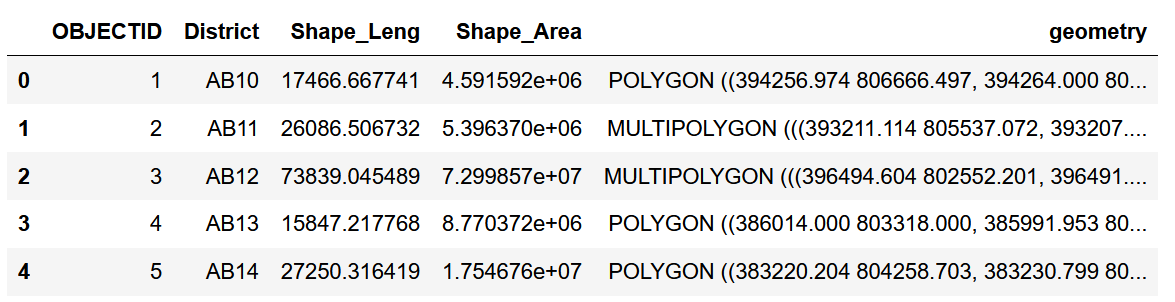
\includegraphics[scale=0.5]{districtcolumns}
\caption{A segment of \texttt{DataFrame} containing district information. Similarly for sector data, with a column
representing postcode sectors.}
\end{center}
\end{figure}
\end{frame}

\begin{frame}{GP Data}
\begin{itemize}
\item{For this example we make use of a few GPs from Lanarkshire (with some modifications):}
\begin{itemize}
\item{Nalagatla Medical Practice}
\item{The Craigallian Avenue Practice}
\item{The Stonelaw Practice}
\item{Ardoch Medical Practice}
\end{itemize}
\item{For the purpose of testing, we also create two hypothetical practices, namely Hypothetical One and Hypothetical Two respectively}
\begin{itemize}
\item{They cover areas defined by a combination of districts and sectors}
\end{itemize}
\end{itemize}
\end{frame}



\begin{frame}{Scotland Total}
\begin{columns}
\begin{column}{0.4\textwidth}
\begin{itemize}
\item{Total admissions in Scotland}
\item{A general decline could be observed}
\end{itemize}
\end{column}

\begin{column}{0.7\textwidth}
%\begin{figure}
%\begin{center}
%\includegraphics[scale=0.45]{scotlandtotal}
%\caption{Combined hospitalisation rates in Scotland.}
%\end{center}
%\end{figure}
\end{column}
\end{columns}
\end{frame}


\section{Conclusion}
\begin{frame}{Summary and Conclusion}
\begin{itemize}
\item{From 2009/10 to 2018/19, a general upward trend could be observed for number of stays, patients and new patients}
\item{Caused by factors such as population number in the 65 or above age group, change in life expectancy}
\item{Using a standard population (EASR), there is a slight declining trend except for the number of new patients}
\item{On the other hand, the overall trend including all age groups in Scotland also shows a general decline}
\end{itemize}
\end{frame}





%\iffalse
\begin{frame}[allowframebreaks]{References} 

%\bibliographystyle{unsrt}
%\bibliographystyle{apalike}

%\bibliographystyle{aasjournal}

%\bibliographstyle{aa_url}
\bibliographystyle{yahapj}

\bibliography{slidescites}
\end{frame}
%\fi

\end{document}
